\documentclass[14pt]{extarticle}

\let\Overrightarrow\overrightarrow
\let\vecarrow\overrightarrow


%other%
\usepackage{graphicx}
\usepackage{float}
\usepackage[margin=0.7in]{geometry}
\usepackage{caption}
\usepackage{csquotes}
\usepackage[export]{adjustbox}
\usepackage{wrapfig}
\usepackage{setspace}
\usepackage{anyfontsize}
\usepackage{titlesec}
\titleformat{\section}{
	\normalfont\fontsize{20}{20}\bfseries}{\thesection}{1em}{}
\titleformat{\subsection}{
	\normalfont\fontsize{17}{20}\bfseries}{\thesubsection}{0.1em}{}
\usepackage{relsize}
%other%



%%\newcommand{\F}{\Oldmathbfcal{F}}
%math%
\usepackage{amsthm}
\usepackage{amssymb}
\usepackage{amsmath}
\usepackage{mathtools}
%%\usepackage[cal = pxtx, scr = dutchcal]{mathalfa}



%\usepackage{unicode-math}
%\newtheorem*{}{\textup{Лемма}}
\newtheorem*{theorem}{\textup{Теорема}}
\newtheorem*{remark}{\textup{Комментарий}}
%\renewcommand\qedsymbol{$\blacksquare$}
%\usepackage{parskip}

\usepackage{pgfplots}
\usepgfplotslibrary{polar}
\usepgflibrary{shapes.geometric}
\usetikzlibrary{calc}


\renewenvironment{proof}
    {\noindent \textit{Доказательство.}\\
	\indent $\square$}
	{ $\blacksquare$\\ }

\newenvironment{solution}
	{\vspace{-4.3mm} \noindent\textbf{Решение.}}


\renewenvironment{remark}
    {\noindent\textbf{Коментарий}}

\usepackage{tikz}
   \usetikzlibrary{calc}

\newcommand{\arc}[0]{
   \tikz [baseline = (N.base), every node/.style={}] {
	  \node [inner sep = 0pt] (N){}; %{$#0$};
      \draw [line width = 0.8pt] plot [smooth, tension=1.3] coordinates {
         ($(N.north west) + (-1.5ex,0.6ex+0.4ex)$)
         ($(N.north)      + (-0.75ex,0+0.4ex)$)
         ($(N.north east) + (0ex,0.6ex+0.4ex)$)
      };
   }
}

\renewenvironment{rcases}
  {\left.\begin{aligned}}
  {\end{aligned}\right\rbrace}

\DeclarePairedDelimiter\abs{\lvert}{\rvert}
\DeclarePairedDelimiter\norm{\lVert}{\rVert}

%\newcounter{example}[section]
\newenvironment{example}[1]{\noindent \textbf{Пример #1.}}

\let\mathb\mathbb


\newcommand{\N}{\mathb{N}}
\newcommand{\Z}{\mathb{Z}}
\newcommand{\R}{\mathb{R}}
\newcommand{\F}{\mathbfcal{F}}
\renewcommand{\P}{\mathbfcal{P}}
\renewcommand{\S}{\mathbfcal{S}}
%\newcommand*{\Z}{\mathbb{Z}}
%math%

%fonts%
\usepackage[russian]{babel}
\usepackage{polyglossia}
\setdefaultlanguage[spelling=modern]{russian}
%\setotherlanguage{english}
\setmainfont{CMU Serif}
\setsansfont{CMU Sans Serif}
\setmonofont{CMU Typewriter Text}  
%\setmathfont{Latin Modern Math}
\usepackage{mathrsfs}
%\DeclareMathAlphabet{\mathcal}{T1}{TX}{m}{n}

\usepackage{unicode-math}


%\let\Oldmathbfcal=\mathbfcal
%\renewcommand{\mathbfcal}{\mumble\Oldmathbfcal}

%%\newcommand{\F}{\Oldmathbfcal{F}}
%%\newcommand{\F}{𝓕}

%\usepackage{fontspec}
\setmathfont{Latin Modern Math}

\DeclareSymbolFont{symbols}{OMS}{cmsy}{m}{n}
\DeclareSymbolFont{bsymbols}{OMS}{cmsy}{b}{n}
\DeclareSymbolFontAlphabet{\mathcal}{symbols}
\DeclareSymbolFontAlphabet{\mathbfcal}{bsymbols}

%\setmathfont[range = {2131}]{AMS}
%\usepackage{amsfonts}
%\usepackage{dsfont}
%fonts%


\begin{document}


Пусть \(T = AC \cap SP\), \(O\) -- центр \((ABC)\). Тогда, 
поскольку \(SB\) -- касательная к \((ABC)\), получаем 
\(\angle BAC = \angle SBP = 
\angle SPB = \angle TPQ\), откуда следует, что 
\(A\), \(B\), \(P\), \(T\) лежат на одной окружности.
С другой стороны, \(\angle APB = 2\angle ACB = \angle AOB\), 
откуда заключаем, что \(A\), \(B\), \(P\), \(O\) лежат на 
одной окружности. Так, все пять точек \(A\), \(B\), \(P\), 
\(T\), \(O\) лежат на \((ABP)\), которую мы обозначим за 
\(\Gamma\). В частности, это означает, 
что \(T\) -- точка пересечения серединного перпендикуляра 
\(\ell\) к \(BC\) и стороны \(AC\). 

Далее, надо как-то разобраться с теми углами, про которые нам 
нужно доказывать утверждение. Оба они \textquote{неудобные}, но 
вот если угол \(BAS\) перебросить не очень понятно как, то вот 
угол \(CAQ\) для этого подходит больше. Вспомним, что 
\(AP = PC\), поэтому давайте отметим точку \(E\) на \(AP\) так, 
что \(PE = PQ\), то есть симметрично \(Q\) относительно серединного перпендикуляра к \(AC\). Тогда понятно, что \(AEQC\) -- р/б 
трапеция, а значит \(\angle CAQ = \angle QEC\). Давайте ещё заметим, что \(\angle XBA = \angle ACB = \angle EQB\). То есть если то, 
что нас просят доказать верно, то треугольники \(ABS\) и \(EQC\) 
подобны. Более того, поскольку они одинаково ориентированы, то 
они вообще должны быть поворотно-гомотетичны. 
Давайте и будем это доказывать. 

\begin{figure}[H]
    \centering
    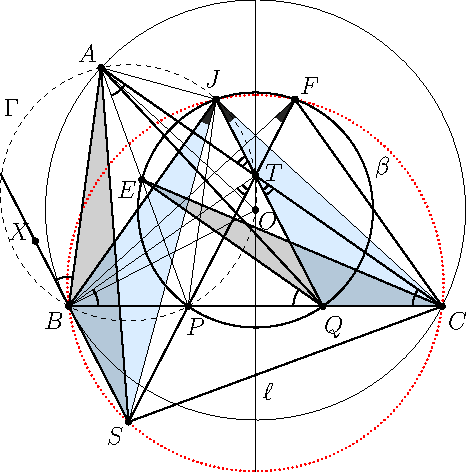
\includegraphics[height=11.4cm]{fig.pdf}
\end{figure}
Окружность \((EPQ)\) обозначим за \(\beta\). Пусть \(J\) -- вторая точка пересечения окружности \(\beta\) с \(\Gamma\). Тогда 
\(J\) -- центр поворотной гомотетии \(\P\), переводящей 
\(AB\) в \(EQ\) (известный факт или счёт углов). 
Значит, осталось доказать, что при этой гомотетии \(S\) 
переходит в \(C\).
%Кроме того, так как \(\angle EJQ = \angle EPB = 
%\angle 

Покажем, что \(J\), \(T\), \(Q\) колинеарны. 
Для этого достаточно доказать, что 
\(\angle JTA = \angle CTQ = \angle PTB\).
Давайте заметим, что \(O\) -- центр \(\beta\). Действительно, 
\(OP = OQ\) из симметрии относительно \(\ell\) и \(OQ = OE\) 
из симметрии относительно серединного перпендикуляра к \(AC\) 
(\(O\) лежит на нём). А значит, \(\beta\) симмерична 
относительно серединного перпендикуляра к \(AB\), так же как и 
\(\Gamma\). А значит, \(J\) и \(P\) симметричны относительно 
серединного перпендикуляра к \(AB\). Мы получили, что 
\(ABPJ\) -- р/б трапеция, что равносильно нужному равенству углов. 
Таким образом, мы доказали, что \(J\), \(T\), \(Q\) колинеарны.
Запомним, что \(ABPJ\) -- р/б трапеция -- этот факт, нам ещё 
пригодится.

Пусть \(F\) -- точка, симметричная \(J\) относительно \(\ell\). 
Докажем теперь, что \(S\), \(B\), \(J\), \(F\), \(C\) лежат на 
одной окружности. Очевидно, что четырёхугольник \(BJFC\) 
вписанный, ведь это 
р/б трапеция. Далее, осталось доказать, что \(\angle SBP = 
\angle SPB = \angle CPF = \angle CFP\), т.е. что \(CF = CP\).
С другой стороны, \(CF = BJ = AP = PC\) (\(BJ = AP\) из равнобедренности 
трапеции). Итого, все указанные выше 5 точек лежат на одной 
окружности.%, которую мы обозначим за \(\xi\).

Осталось заметить, что \(\angle QJC = \angle PFB = \angle SJB\) и
\(\angle JCB = \angle JSB\), откуда получаем, что \(J\) -- 
центр поворотной гомотетии \(\F\), которая переводит \(BS\) в 
\(QC\). Остаётся заметить, что коэффициенты обоих поворотных 
гомотетий 
\(\P\) и \(\F\) равны \(JB/JQ\), а их углы равны \(\angle BJQ\).
Откуда получаем, что \(\P\) и \(\F\) на самом деле одна и та же 
поворотная гомотетия \(\S\). Таким образом, \(\S\) переводит \(AB\) в \(EQ\) 
и \(BS\) в \(QC\). То есть \(\S\) -- искомая поворотная гомотетия, 
переводящая треугольник \(ABS\) в треугольник \(EQC\). Поэтому 
\(\angle BAS = \angle QEC = \angle QAC\), что и требовалось.
%а это равносильно тому, что \(JP \parallel AB\)

\end{document}
